\newpage
\section{Metodologia Experimental}

\subsection{Materiais}

Para a realização do experimento foi utilizado o software Simulink do pacote Matlab.

O experimento foi realizado em três partes. De início, foi estudado o comportamento da modulação Delta. Em seguida, foi analisado o diagrama de olho e por ultimo, a recepção com detector coerente.

\subsection{Modulação Delta}
Na primeira atividade, foi montado o circuito da figura \ref{fig:deltamod} com ajuda do roteiro que continha todos os parâmetros necessários para configurar os blocos.

\begin{figure}[H]
    \centering
    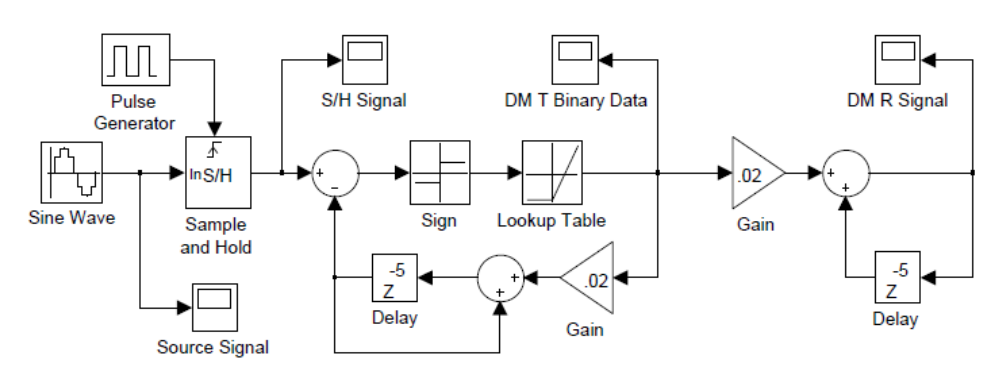
\includegraphics[scale=0.3]{deltamod}
    \caption{Diagrama do sistema com modulação delta.}
    \label{fig:deltamod}
\end{figure}

Foram obtidos os gráficos em todos os osciloscópios e foi verificado o atraso na saída.

\subsection{Modulação Delta: erro de quantização}
Na segunda atividade, foi montado o circuito da figura \ref{fig:deltamoderro} com ajuda do roteiro que continha todos os parâmetros necessários para configurar os blocos.

\begin{figure}[H]
    \centering
    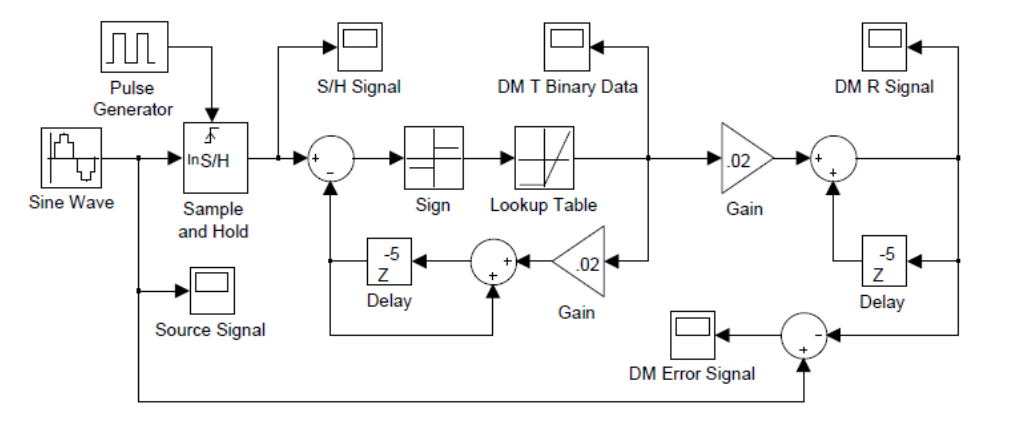
\includegraphics[scale=0.3]{deltamoderro}
    \caption{Diagrama do sistema com modulação delta para capturar o erro de quantização.}
    \label{fig:deltamoderro}
\end{figure}

Foi obtido o gráfico que mostra o erro de quantização.


\subsection{Modulação Delta: distorção de inclinação de sobrecarga}
Na terceira atividade, foi montado o circuito da figura \ref{fig:deltamoddistorcao} com ajuda do roteiro que continha todos os parâmetros necessários para configurar os blocos.

\begin{figure}[H]
    \centering
    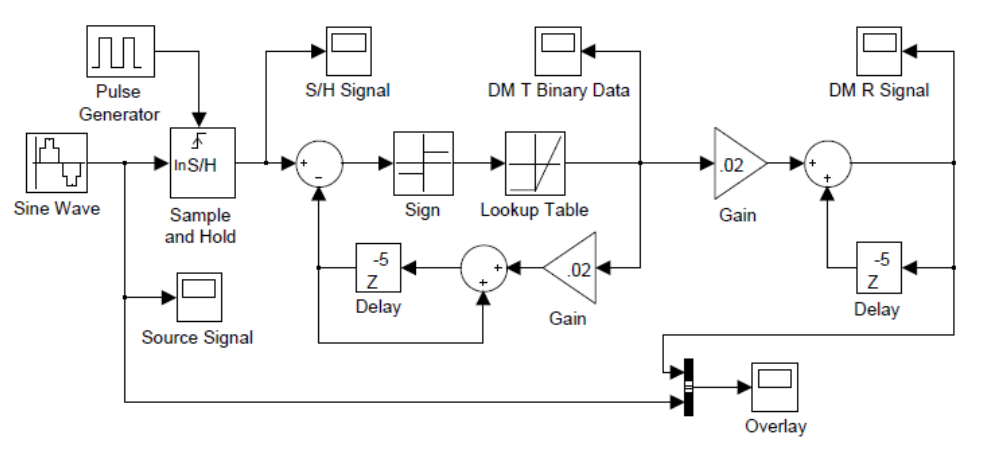
\includegraphics[scale=0.3]{deltamoddistorcao}
    \caption{Diagrama do sistema com modulação delta para capturar a distorção.}
    \label{fig:deltamoddistorcao}
\end{figure}

Foi obtido o gráfico que mostra a distorção de sobrecarga.

\subsection{Modulação Delta: ruído granular}
Na quarta atividade, foi montado o circuito da figura \ref{fig:ruido} com ajuda do roteiro que continha todos os parâmetros necessários para configurar os blocos.

\begin{figure}[H]
    \centering
    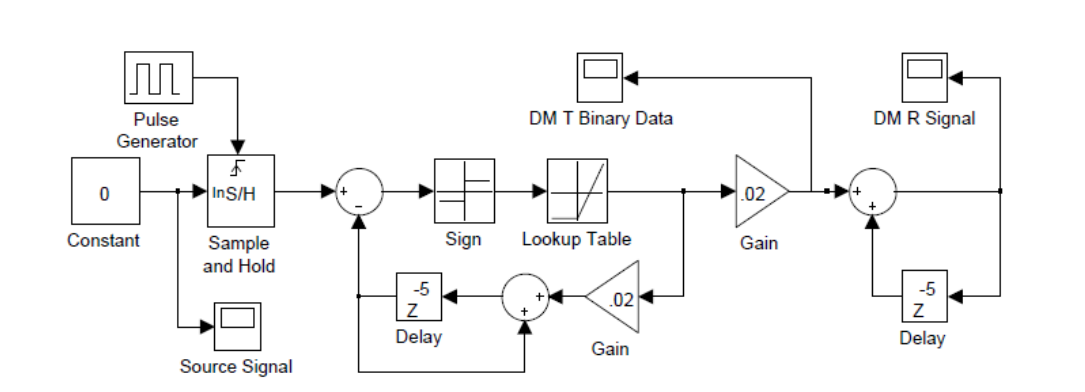
\includegraphics[scale=0.3]{ruidogranular}
    \caption{Diagrama do sistema com modulação delta para capturar o ruído granular.}
    \label{fig:ruido}
\end{figure}

Foi obtido o gráfico que mostra o ruido granular.

\subsection{Diagrama de olho}
Na quinta atividade, foi montado o circuito da figura \ref{fig:eyediagram1} para os valores de variância de $\sigma =0 V^2$, $\sigma =0.5 V^2$ e $\sigma =6 V^2$, com ajuda do roteiro que continha todos os parâmetros necessários para configurar os blocos.

\begin{figure}[H]
    \centering
    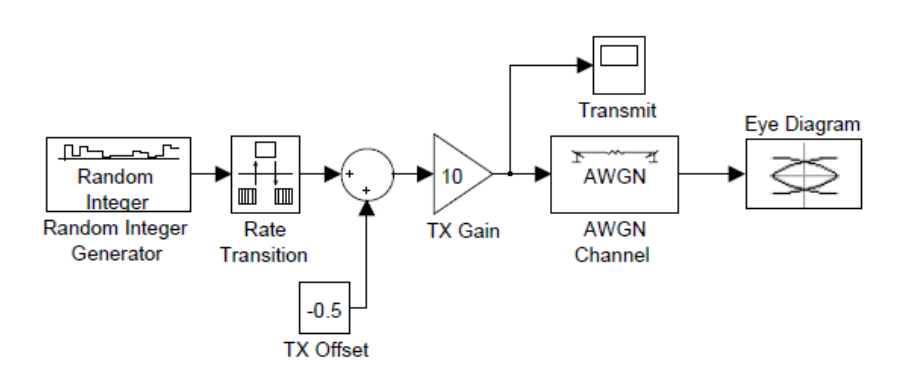
\includegraphics[scale=0.3]{simulinkeyediagram}
    \caption{Diagrama para obter o diagrama de olho.}
    \label{fig:eyediagram1}
\end{figure}

Foi obtido o gráfico que mostra o diagrama de olho.


\subsection{Diagrama do olho:Redução da Largura de Banda, Jitter e Redução da Largura de Banda e Jitter}
Na sexta atividade, foi montado o circuito da figura \ref{fig:eyediagram2}, variando o parâmetro Maximum no Uniform Random Number de 0.0005 para 0.000075.

\begin{figure}[H]
    \centering
    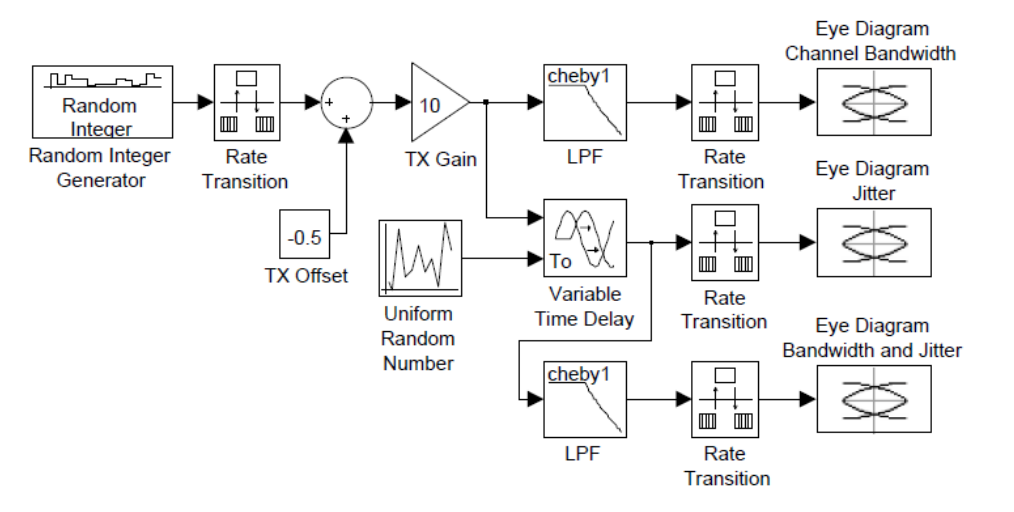
\includegraphics[scale=0.3]{eyediagram2}
    \caption{Diagrama para obter o diagrama de olho com variação do Jitter e da largura de banda.}
    \label{fig:eyediagram2}
\end{figure}

Foi obtido o gráfico que mostra o diagrama de olho para cada uma das saídas.


\subsection{Receptor em Banda Passante Ótimo: O Receptor de Correlação}
Na sétima atividade, foi montado o circuito da figura \ref{fig:receptorcorr} com ajuda do roteiro que continha todos os parâmetros necessários para configurar os blocos.

\begin{figure}[H]
    \centering
    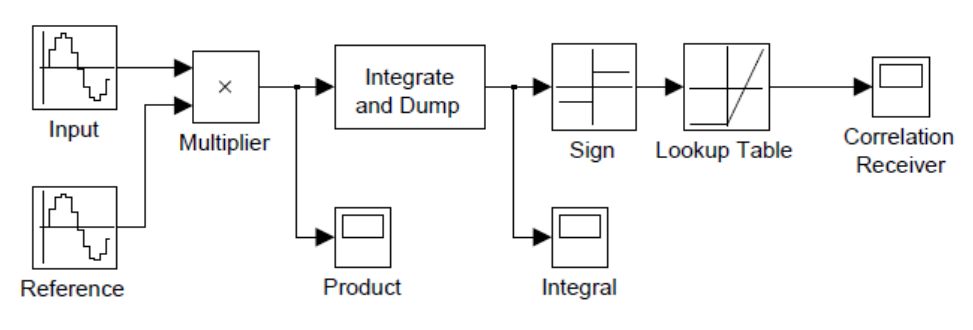
\includegraphics[scale=0.3]{recpcorrelacao}
    \caption{Diagrama do receptor de correlação simples.}
    \label{fig:receptorcorr}
\end{figure}

Foram obtidos os gráficos onde possui osciloscópio.


\subsection{Receptor de Correlação para Sinais Assimétricos em Banda Passante}
Na oitava atividade, foi montado o circuito da figura \ref{fig:rec2} com ajuda do roteiro que continha todos os parâmetros necessários para configurar os blocos.

\begin{figure}[H]
    \centering
    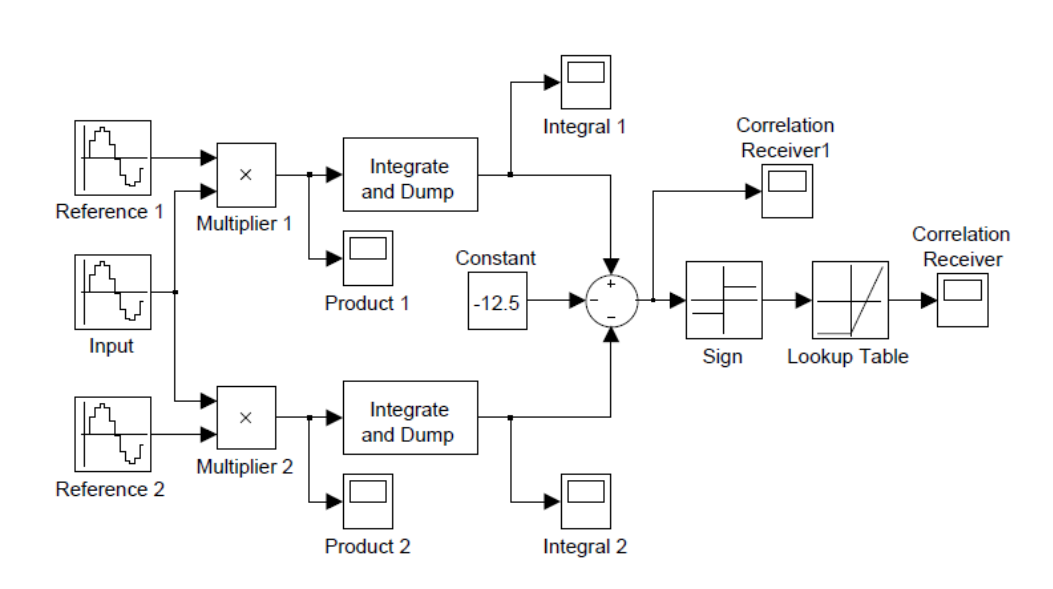
\includegraphics[scale=0.3]{receptor2}
    \caption{Diagrama do receptor de correlação com sinais assimétricos.}
    \label{fig:rec2}
\end{figure}

Foram obtidos os gráficos onde possui osciloscópio.